\section{Scaling of the error compared to discretization}
The charge density is represented on a discretized grid and due to this a numerical solution
will have an inherent error.
The error will be of second order, \(\order{h^{-2}}\), dependent on the
stepssize, \(\Delta x\), due to the first order solver, see \cref{sec:GSRB}.

To investigate that the error of the solver follows a second order improvement
as the stepsize decreases we construct a sinusoidal \(\rho\) as a test case.

\begin{equation}
    \rho(x) = \sin{\left(\frac{x}{2\pi}\right)}; \qquad x\epsilon[0,2\pi] \label{eq:sinus_errorScaling}
\end{equation}

This \(\rho\) is analytically solvable for the Poisson equation so we can compute the
\(2\)-norm of the error, \(\norm{err}_2\). Then we gradually decrease the stepsize
and compare the norm of numerical solutions. Since the normalization in PINC
is normally done outside the multigrid solver, \(rho\) had to be suitably scaled
to the stepsize. We expect the error to be proportional to the squared stepsize, \(err(h) \approx Ch^2\), where \(C\) is a constant dependent on the geometry of the problem.
By taking the logarithm we obtain

\begin{equation}
    \log(err(h)) = 2\log(Ch)
\end{equation}

Fig. \ref{fig:errorScaling} shows the
the measured error when solving the sinusoidal charge distribution, \cref{eq:sinus_errorScaling},
for both the potential, \(\phi\), and the electric field, \(E_x\).
The problem was solved with different discretizations on a \(3\)-dimensional domain,
starting at \([8,8,8]\) doubling the grid points each time. The slope on the logarithmic plots
was in both cases found to be \(2.00\), showing a second order error scaling \(\order{h^{-2}}\).
The same test was also performed in \(1\) and \(2\) dimensional cases, with varying
subdomain configurations and with the sinus shape along the other axes.

\begin{figure}
    \centering
    \begin{subfigure}[b]{\textwidth}
        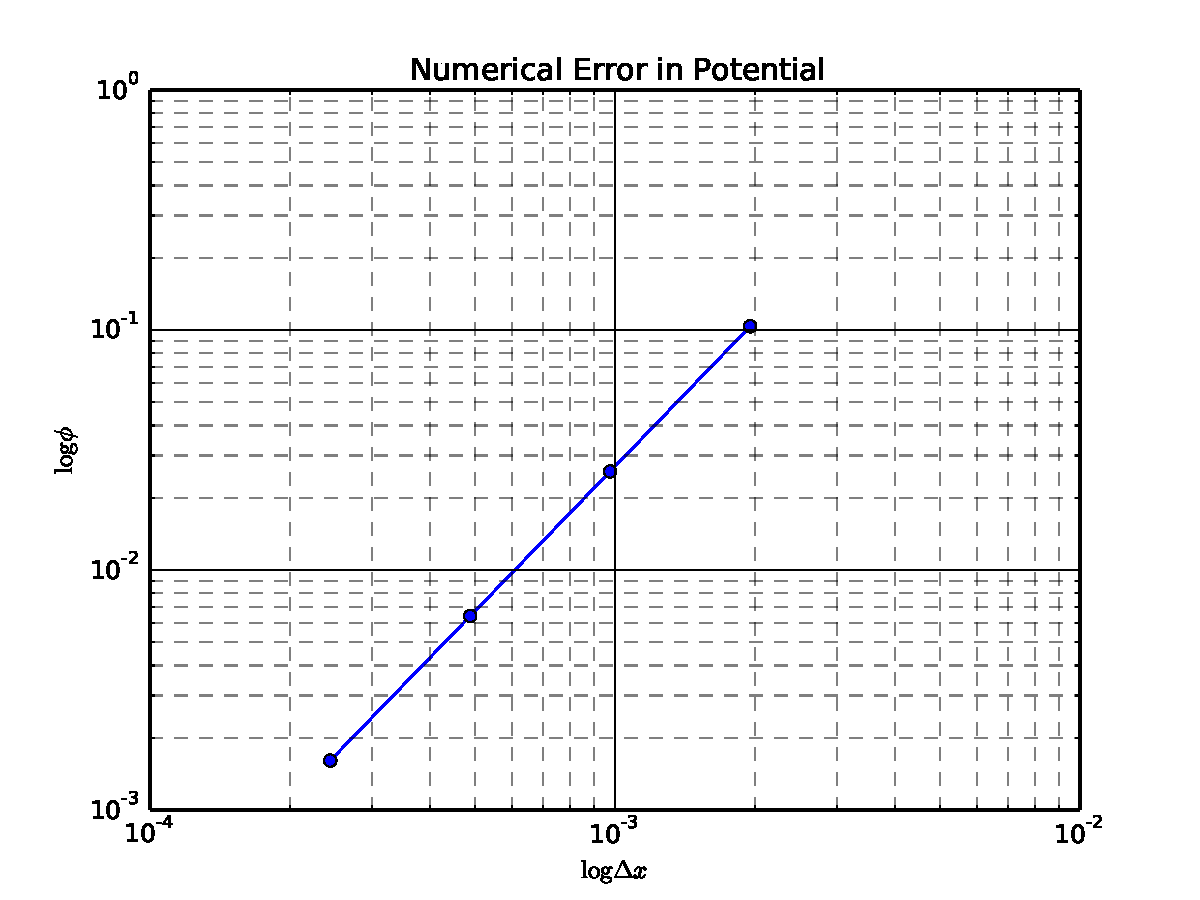
\includegraphics[width = \textwidth]{figures/verification/errorScaling/errorloglogPotential}
    \end{subfigure}
	\begin{subfigure}[b]{\textwidth}
		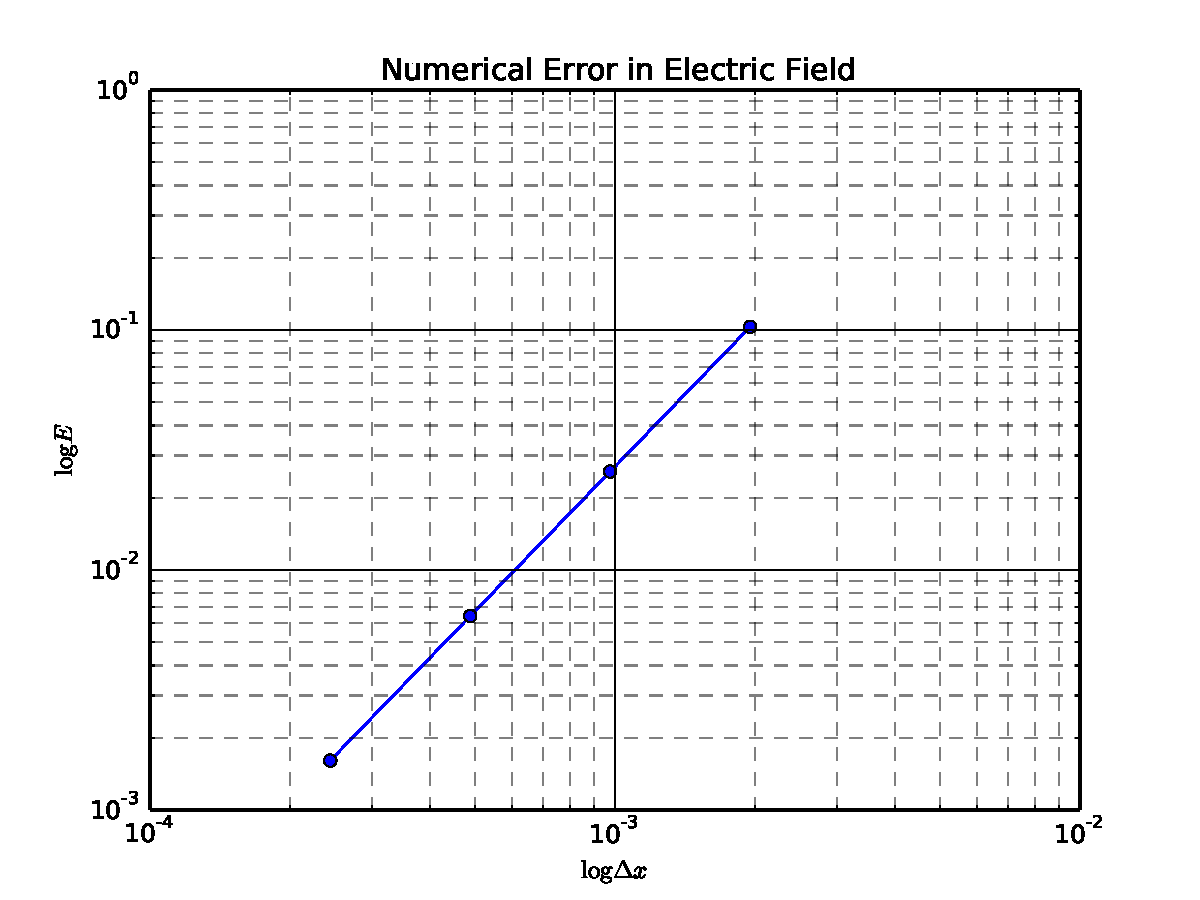
\includegraphics[width = \textwidth]{figures/verification/errorScaling/errorloglogE}
	\end{subfigure}
    \caption{Logarithmic plot of the 2-norm of the error of the potential \(\phi\), top figure, and the
    x-component of the electric field. The solver was run on a scaled sinus-shaped charge distribution.
    Both of the plots show a straight line of the error, on the logarithmic plots, with a slope
    of \(2.00\). This corresponds to the error scaling with order \(-2\) as a function of the
	stepsize as expected. All the units are in PINC normalized units.}
    \label{fig:errorScaling}
\end{figure}
